\documentclass[a4paper]{book}
\usepackage[utf8]{inputenc}
\usepackage{graphicx}
\usepackage{amsfonts}
\usepackage{amsmath}
\usepackage{amssymb}
\usepackage{titling}
\usepackage{hyperref}
\usepackage{xcolor}
\usepackage{pagecolor}
\usepackage{eso-pic}
\usepackage{float}

\newcommand\BackgroundPic{%
	\put(0,0){%
		\parbox[b][\paperheight]{\paperwidth}{%
			\vfill
			\centering
			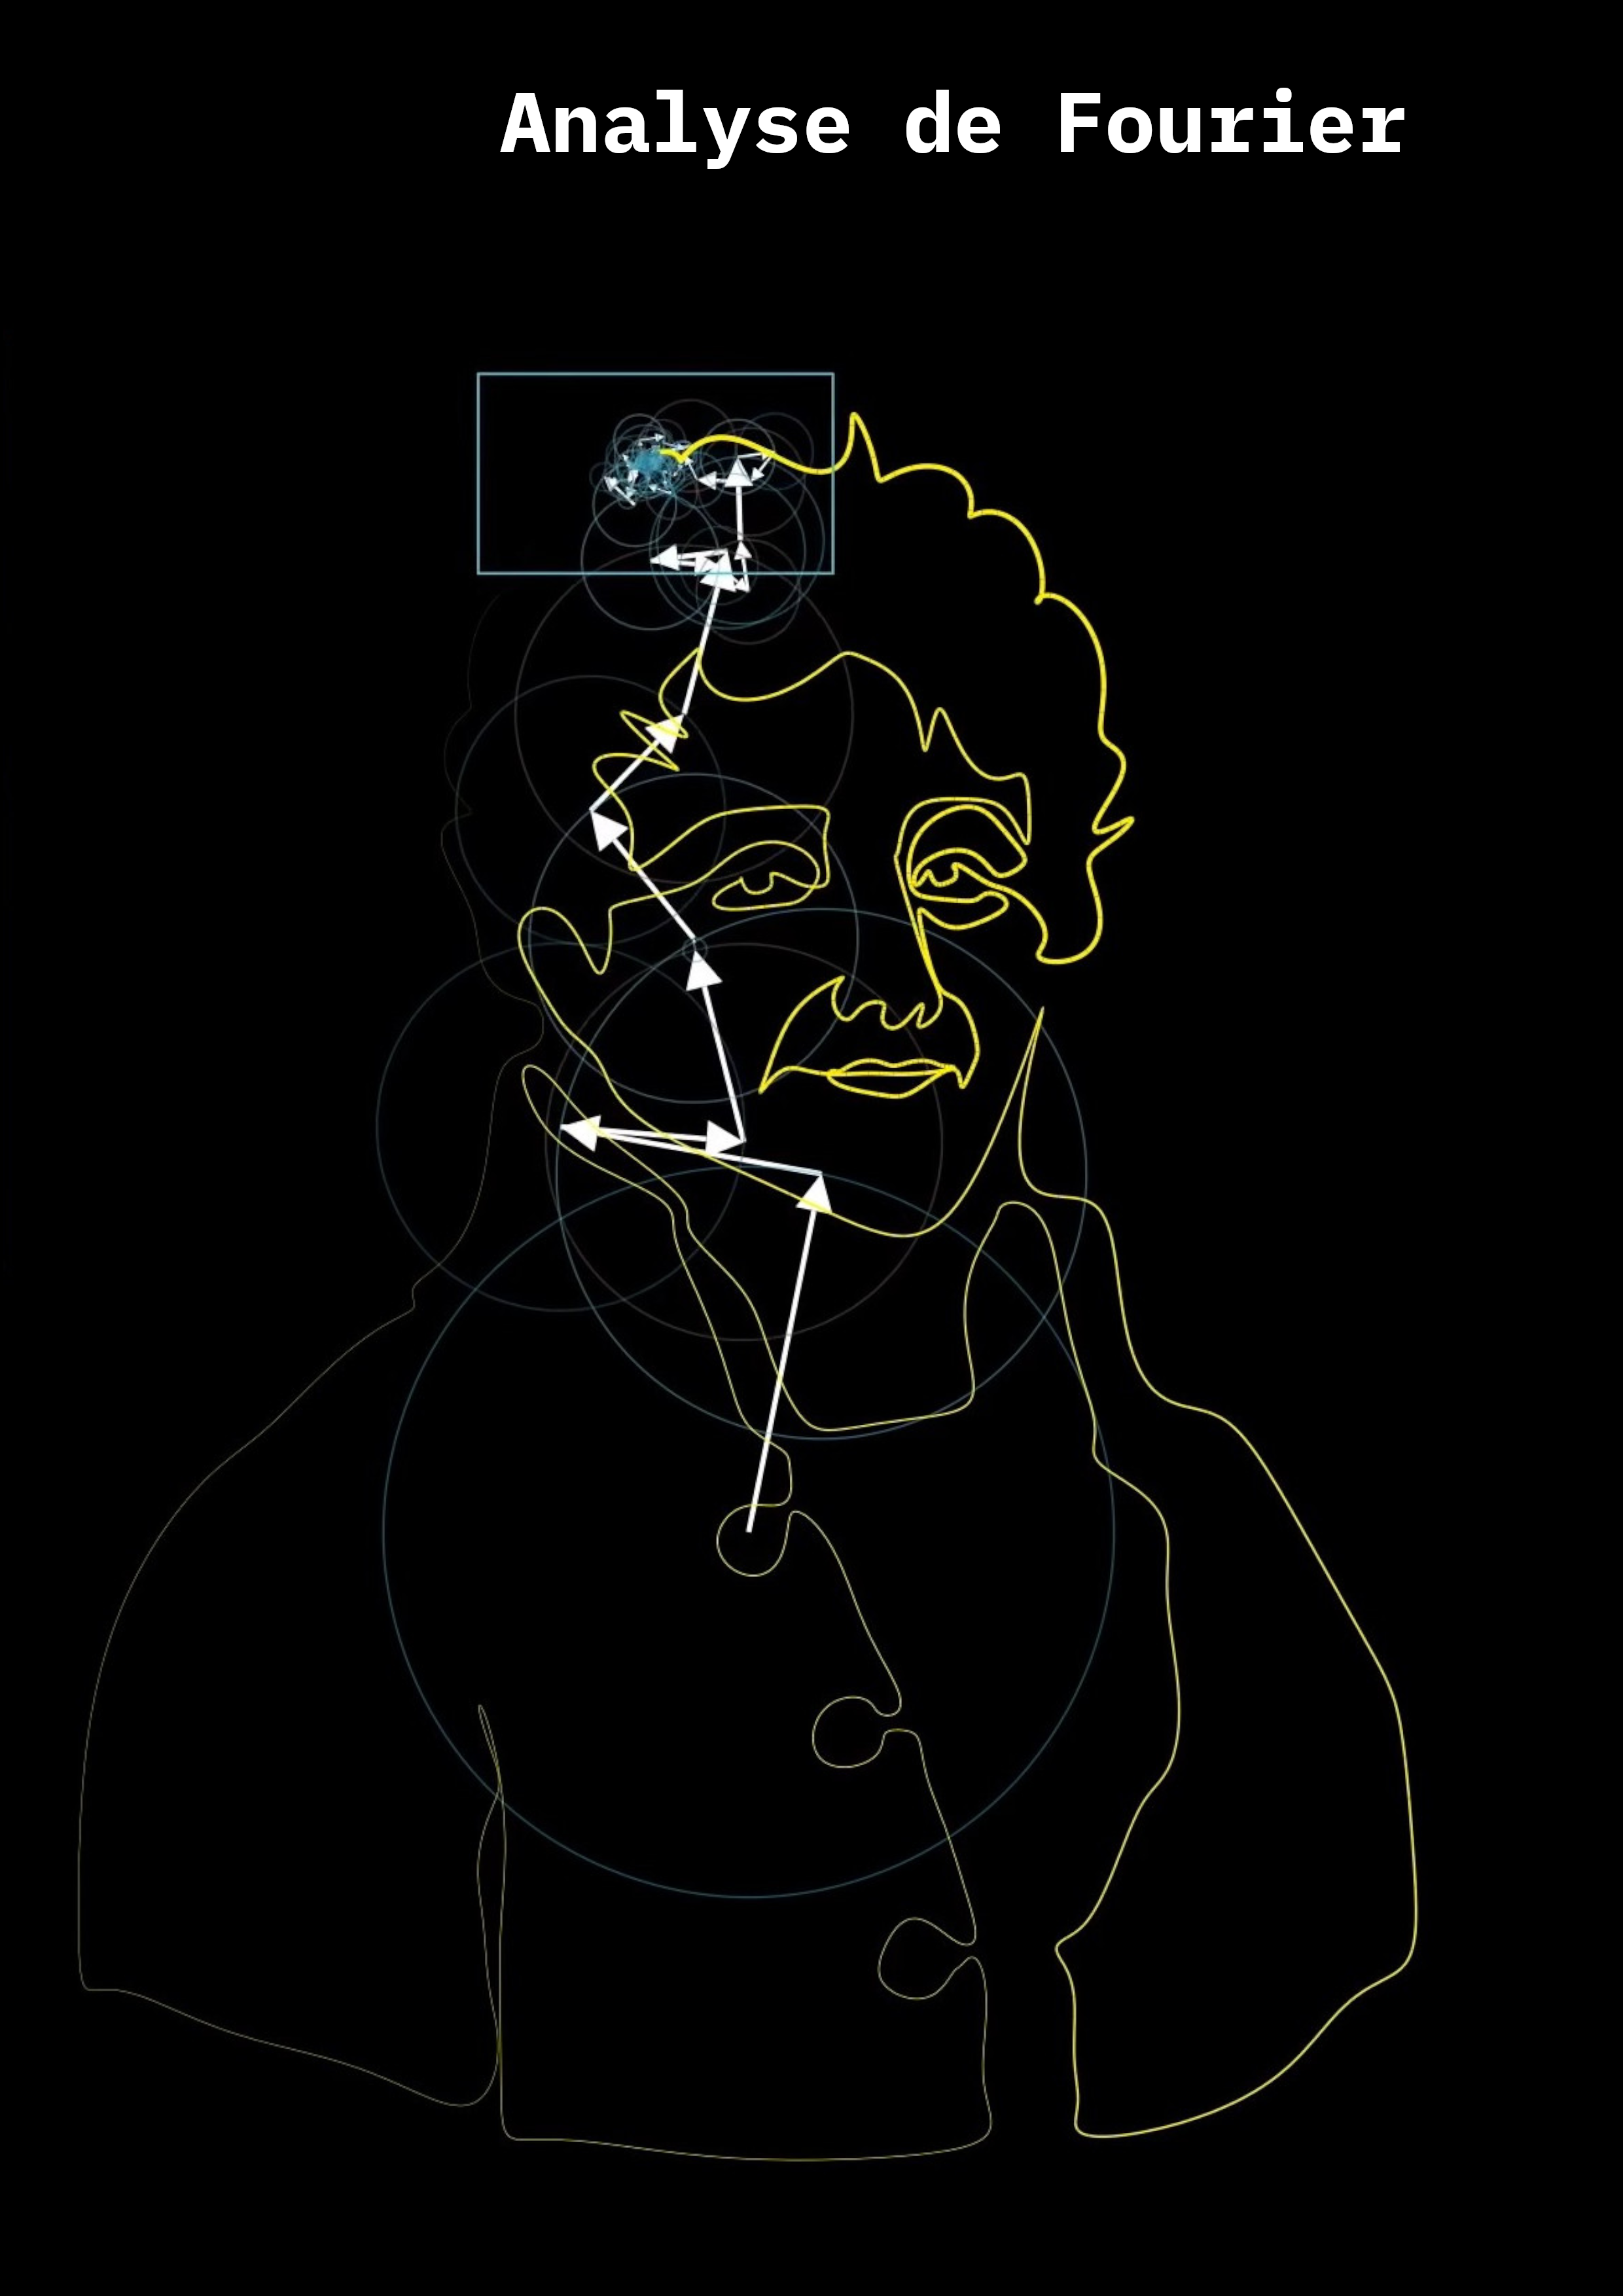
\includegraphics[width=\paperwidth,height=\paperheight,%
			keepaspectratio
			]{background.png}%
			\vfill
		}
	}
}

\graphicspath{ {./img/}, {./img/doppler/} }
\hypersetup{
	colorlinks=true,
	urlbordercolor=black,
	linkcolor=black,
	filecolor=magenta,      
	urlcolor={red!80!black},
}

%\title{Analyse de Fourier}
%\author{Philippe Krejci}
\date{}

\begin{document}
\AddToShipoutPicture*{\BackgroundPic}
\maketitle
\clearpage

\tableofcontents


\chapter{Abstract}
\paragraph{L'objectif final de ce cours est de comprendre les \underline{Transformée de
Fourier}. Savoir d'où elles viennent, en comprendre ses expressions et ce
qu'elles permettent de faire.}

\newline
La physique a pour objectif l'étude des phénomènes naturelles. \emph{Ici nous nous
concentrerons sur le traitement du signal}.

Le \textbf{signal} est une mesure physique observable d'un phénomène le plus
souvent électrique, acoustique ou optiques. L'étude par Fourier permet de
réinterpréter le signal, qui est une fonction complexe, en une somme de
fonctions périodiques qui en permet une simplification de calcul. \textbf{Plus
de détails dans le chapitre suivant s'intitulant \underline{Introduction
Visuelle à Fourier}}.

\newline
\vspace{5mm}
Pour le moment, ce qui suit n'est que présenté, et sera détaillé plus tard dans
le chapitre \textbf{Transformée de Fourier}.
Soit $\hat{f} : \mathbb{R} \mapsto \mathbb{C}$, sans supposé périodicités de
$\hat{f}$,
\begin{equation}
	\hat{f}(x) = (2\pi)^{-n} \int_{\mathbb{R}^n} e^{ix\zeta}f(\zeta) \, d\zeta
\end{equation}
Où $f$ défini dans $\mathbb{R}^n$, s'appelle la transformée de Fourier de
$\hat{f}$,
\begin{equation}
	f(x) = \int_{\mathbb{R}^n} e^{-ix\zeta}\hat{f}(x) \, dx
\end{equation}
L'expression $(1)$ exprime $\hat{f}$ comme superposition indexé par \zeta, de
fonction simple : \\
$x \mapsto e^{ix\zeta}$ qui oscillent à la fréquence $2\pi|\zeta|$ étant affecté
à l'amplitude $|s(\zeta)|$ et d'une phase $\arg{s(\zeta)}$.

Ainsi, ce lien permet d'exprimer $\hat{f}$ en fonction de $f$ et vice-versa. On
observe une \textbf{dualité importante entre analyse de l'amplitude et l'analyse
fréquentiel.} (En \underline{mécanique quantique} les rôles joués par $\hat{f}$ et $f$
sont \underline{parfaitement symétrique}).

À travers ce cours nous allons parcourir les chapitres suivants :
\begin{itemize}
	\item \textbf{Fonction holomorphe d'une variable complexe} : permettra
		d'introduire les coefficients de Fourier
	\item \textbf{Espace fonctionnel et convergent}
	\item \textbf{Espace hilbertiens} : permet en replaçant le signal dans
		un nouvelles espace de simplifier les calculs et d'attaquer les
		fonctions de carré sommable
	\item \textbf{Série de Fourier} : est  une étape intermédiaire pour
		manipuler par la suite les intégral en question
	\item \textbf{Transformée de Fourier}
\end{itemize}

\chapter{Introduction Visuelle à Fourier}

\section{Enroulement du signal sur le cercle complexe}
\begin{figure}[h]
	\centering
	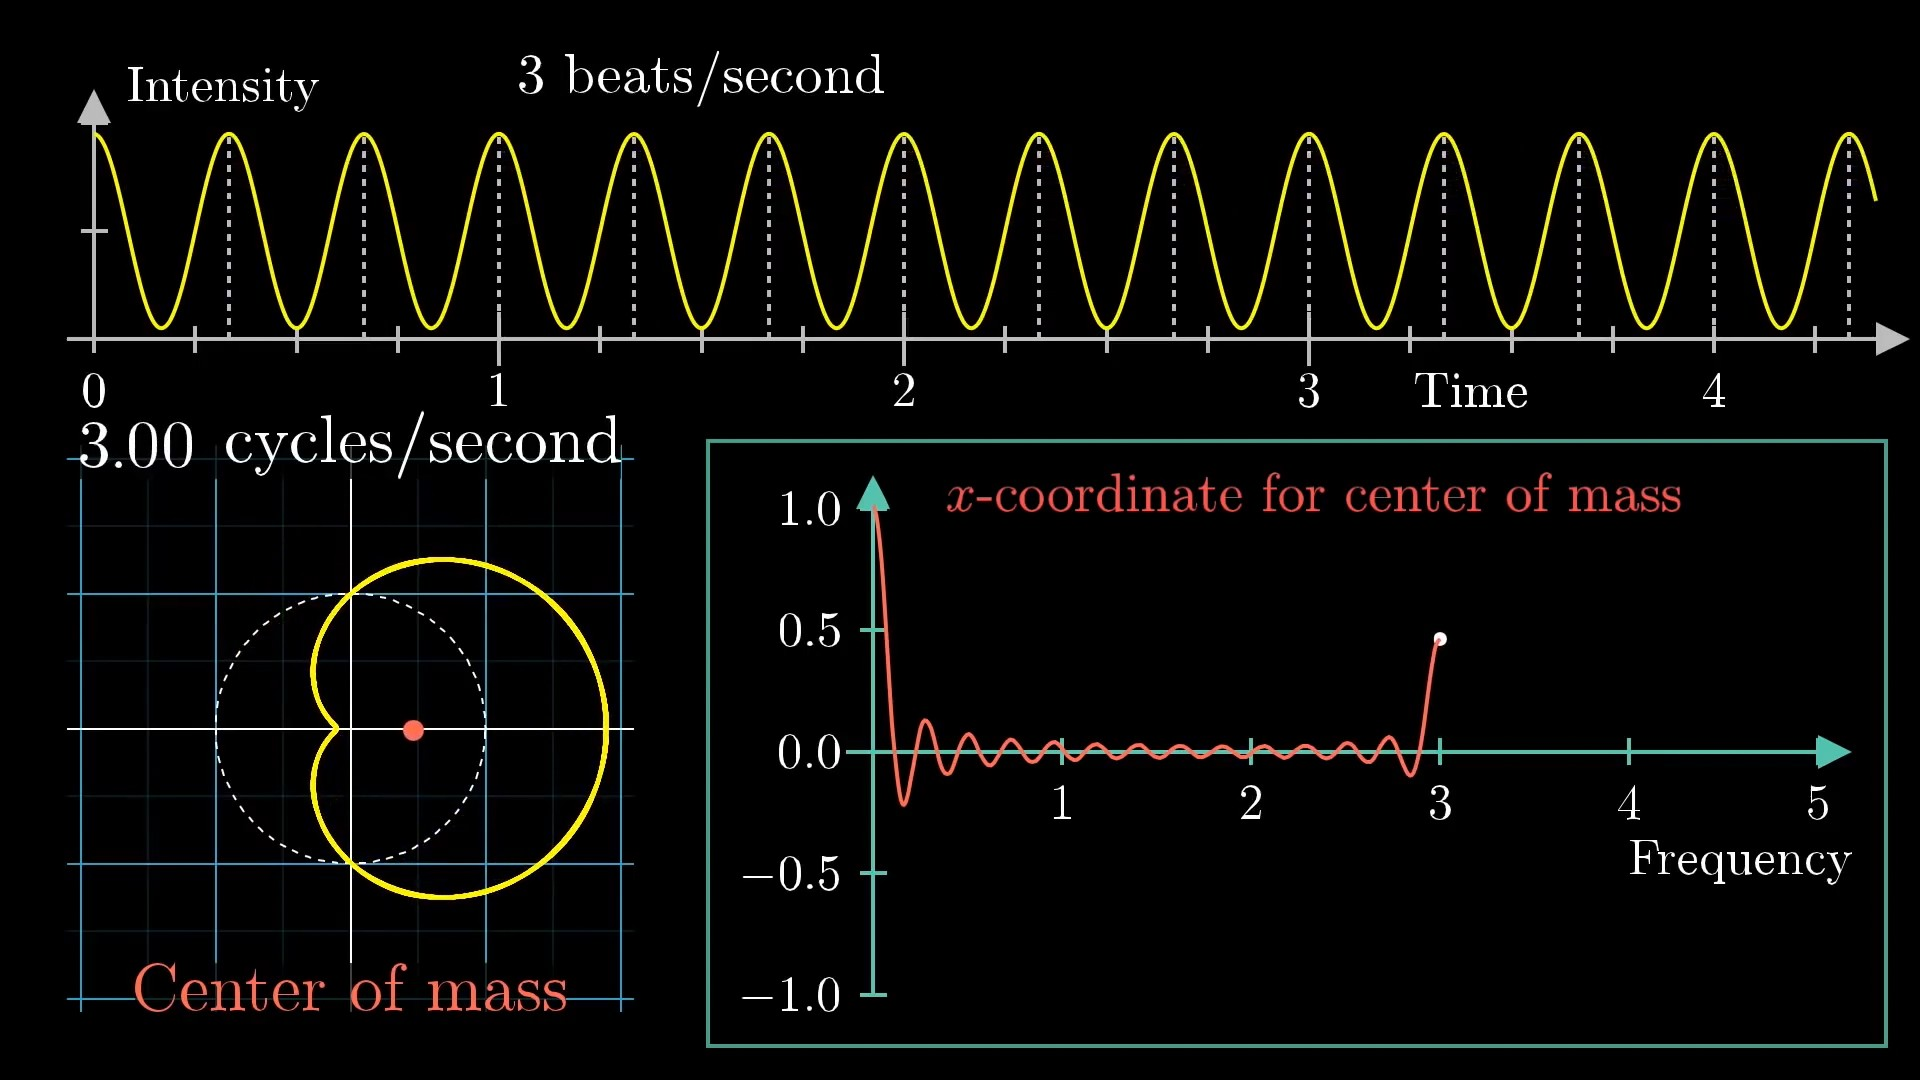
\includegraphics[scale=0.2]{visu_fourier.jpg}
	\caption{Enroulement du signal sur le cercle
	complexe : © 3blue1brown }
\end{figure}


Pour comprendre l'idée général de la Transformé de Fourier, il faut
\textbf{impérativement} regarder cette vidéo : 
\href{https://www.youtube.com/watch?v=spUNpyF58BY}{3blue1brown : But 
what is the Fourier Transform? A visual introduction.}

\underline{Point clefs à retenir}
\begin{itemize}
	\item \textbf{Objectif} : le signal est une fonction complexe.
		L'objectif est de le représenter d'une manière plus simple.
		\underline{Or} selon Fourier, une fonction quelconque peut se
		représenter sous la sommes de plusieurs fonctions périodiques.
	\item Toutes fonctions périodiques sont représentables sur un cercle
		complexe "enroulement d'une fonction". En effet, liée à leur
		caractéristique d'être périodique, elle peut se représenter sur
		un cercle où la vitesse parcourut sur un  cycle correspondrai à 
		la fréquence du signal que l'on étudie.
	\item Comment "enrouler la fonction" ? Imaginons que l'on a un vecteur
		qui est en rotation sur un cercle unitaire en fonction du temps.
		Nous lui associons, le module à l'amplitude du signal à
		l'instant $t$ correspondant. La vitesse à laquelle un tour est
		éffectué en parcourant le cercle, s'intitule un cycle. Ainsi un
		cycle par unité de temps s'intitule une fréquence. Cette
		représentation s'effectue sur un \underline{cercle complexe}
		pour ainsi simplifier la représentation des coordonées de
		points, où l'axe des absices correspond à celui de la partie
		réel, et l'axe des ordonées à celui de la partie imaginaire.
		Soit $(x,y) \mapsto x+iy$.
	\item \textbf{Remarque} : à ce stade, on constate qu'il y a deux
		fréquences différentes. La première, correspond à celle du
		signal, càd au bout de combien de temps le plus motifs se
		répète. La seconde, celle sur le cercle détaillés au point
		précédent. Pour le moment ces deux fréquence sont dissocier.
	\item En observant le point de gravité (qui sera détaillé dans le
		chapitre \textbf{Fonction holomorphe d'une variable complexe})
		on remarque que lorsque la fréquence
		de représentation sur le cercle coïncide avec celle du signal
		donné alors, la coordonnée $x$ a un comportement spécifique.
		Cette dernière est décentré. En effet, tant que les fréquences
		ne coïncide pas, le point de gravité gravite aux alentours du
		point $z_{0} = 0+i0$.
	\item L'objectif de la Transformé de Fourier est de repérer ce
		changement de comportement. Il permet ainsi d'obtenir les
		différentes fréquences que comporte ce signal.
	\item Ainsi le signal est exprimable par les différentes fréquences qu'il
		comporte.
\end{itemize}

\underline{Transcription Mathématiques} : Cette représentation permet de
simplifier le signal, comme prévu. Voici ce que l'on obtient par étapes, pour
obtenir le \textbf{centre de gravité} en question. \\
Premièrement, rappelons que l'équation du cercle complexe s'écrit sous cette
forme $e^{2 \pi i t}$. Pour représenté la fréquence $f$, cela équivaut à accélérer
ou ralentir le temps, autrement dit, appliqué un facteur au temps qui lui
s'écoule de la même manière :
\begin{equation}
	e^{- 2 \pi i t f}
\end{equation}
\underline{Remarque} : par convention dans le contexte de Fourier le sens est
négatif.\\
Maintenant, associons l'amplitude du signal $g(t)$ au module :
\begin{equation}
	g(t) e^{- 2 \pi i t f}
\end{equation}
À ce niveau là, nous venons d'exprimer la coordonnée $(x,y)$ d'un point
correspondant à l'enroulement du signale en question à l'instant $t$.\\
Pour obtenir le \underline{point de gravité}, il faut obtenir la moyenne de tout
les points :
\begin{equation}
	\frac{1}{N} \sum_{k=0}^{N} g(t_{k}) e^{- 2 \pi i t_{k} f}
\end{equation}
Ainsi, pour obtenir le meilleur point de gravité, il faut tendre $N$ vers
$\infty$. Ce qui revient à écrire :
\begin{equation}
	\frac{1}{t_{2} - t_{1}} \int_{t_{1}}^{t_{2}} g(t) e^{2 \pi i t f} \, dt
\end{equation}
Nous venons d'obtenir l'équation du \textbf{point de gravité}.\\
Mais la transformée de Fourier ne correspond qu'à la partie intégral, soit :
\begin{equation}
	\int_{t_{1}}^{t_{2}} g(t) e^{2 \pi i t f} \, dt
\end{equation}
\textbf{Remarque} : l'intérêt réside dans le fait que l'extraction de fréquence
sera plus facile. En effet, sans la fraction, nous n'obtenons plus une moyennes,
et ainsi nous obtenons une accumulation; lorsque le point de gravité se
décentrera alors la différence sera plus importante, surtout si l'on effectue
plusieurs tours.

\section{Cas appliqué : Doppler }

Maintenant étudions un cas spécifique d'application de Fourier, pour cela voir
\href{https://www.youtube.com/watch?v=MBnnXbOM5S4}{3blue1brown : more general 
uncertainty principle, quantum}. \\ \break

Nous allons admettre le \underline{Principe d'incertitude de Heisenberg} (en
théorie quantique) pour la suite, (et nous allons appercevoir que nous 
retrouveron l'analyse de Fourier).\\
\underline{Que dit ce théoreme ?} Plus nous sommes précis sur la position d'une
particule, moins nous en savons sur son momentum (\emph{càd ici, fréquence}).
Et vice-versa.

\subsection{Environnement simple}
\begin{figure}[htb!]
	\centering
	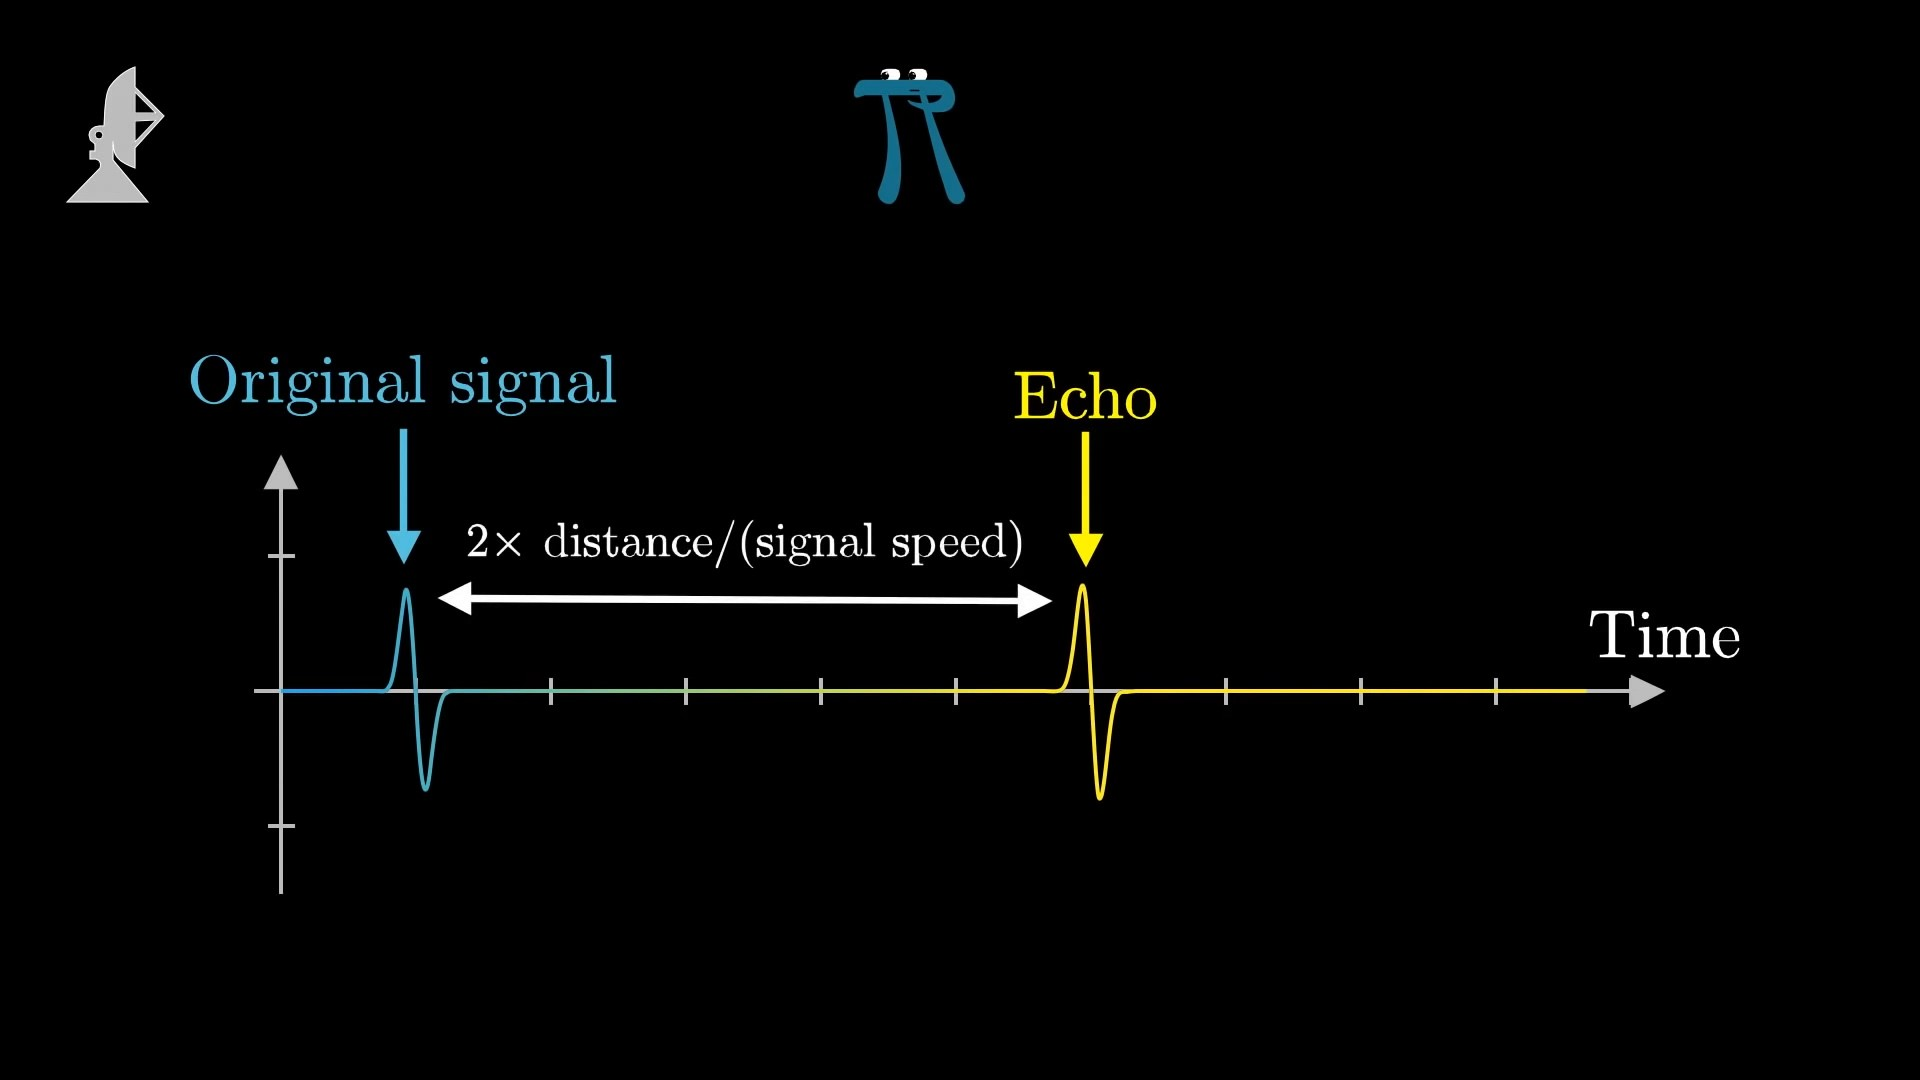
\includegraphics[scale=0.2]{env_simple.jpg}
	\caption{Étude de Doppler dans un environnement
	simple : ©3blue1brown }
\end{figure}
Le \underline{radar} émet une impulsion simple. Lorsque cette onde entre en
collision avec la \underline{cible}, elle est retourné au radar qui la capte. À
partir du delta nous pouvons déduire la distance de la cible en question.

\subsection{Détermination du la vitesse}
\begin{figure}[H]
	\centering
	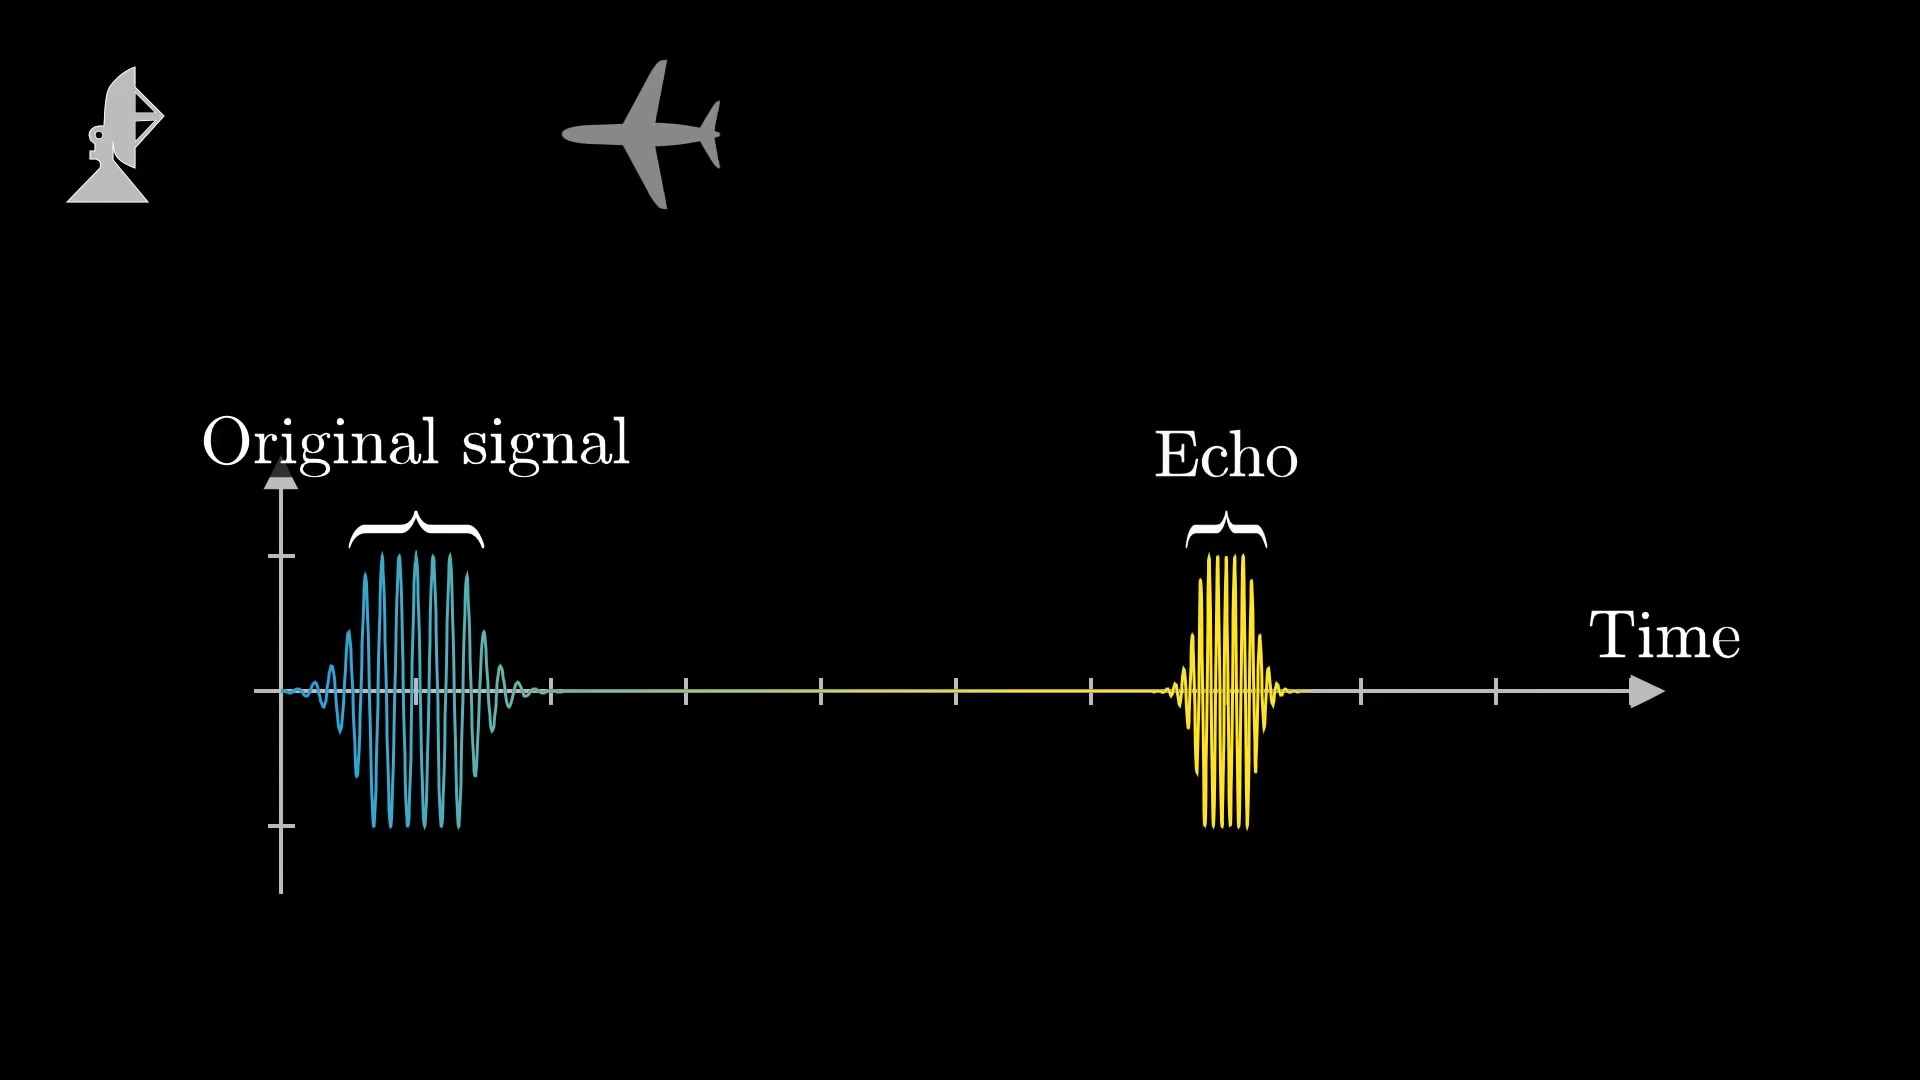
\includegraphics[scale=0.2]{env_vitesse.jpg}
	\caption{Détermination de la vitesse par compression d'onde
	: ©3blue1brown }
\end{figure}
\emph{Dans le cas précèdent nous obtenions que très peu d'information}.
Maintenant, le \underline{radar} envoie un signal (comportant une fréquence).
Ce signal rentre en collision contre la \underline{cible}. Si la cible
avance[/s'eloigne] vers[/du] le radar, alors le signal de retour sera 
compressé[/décompressé]. \\

\begin{figure}[H]
	\centering
	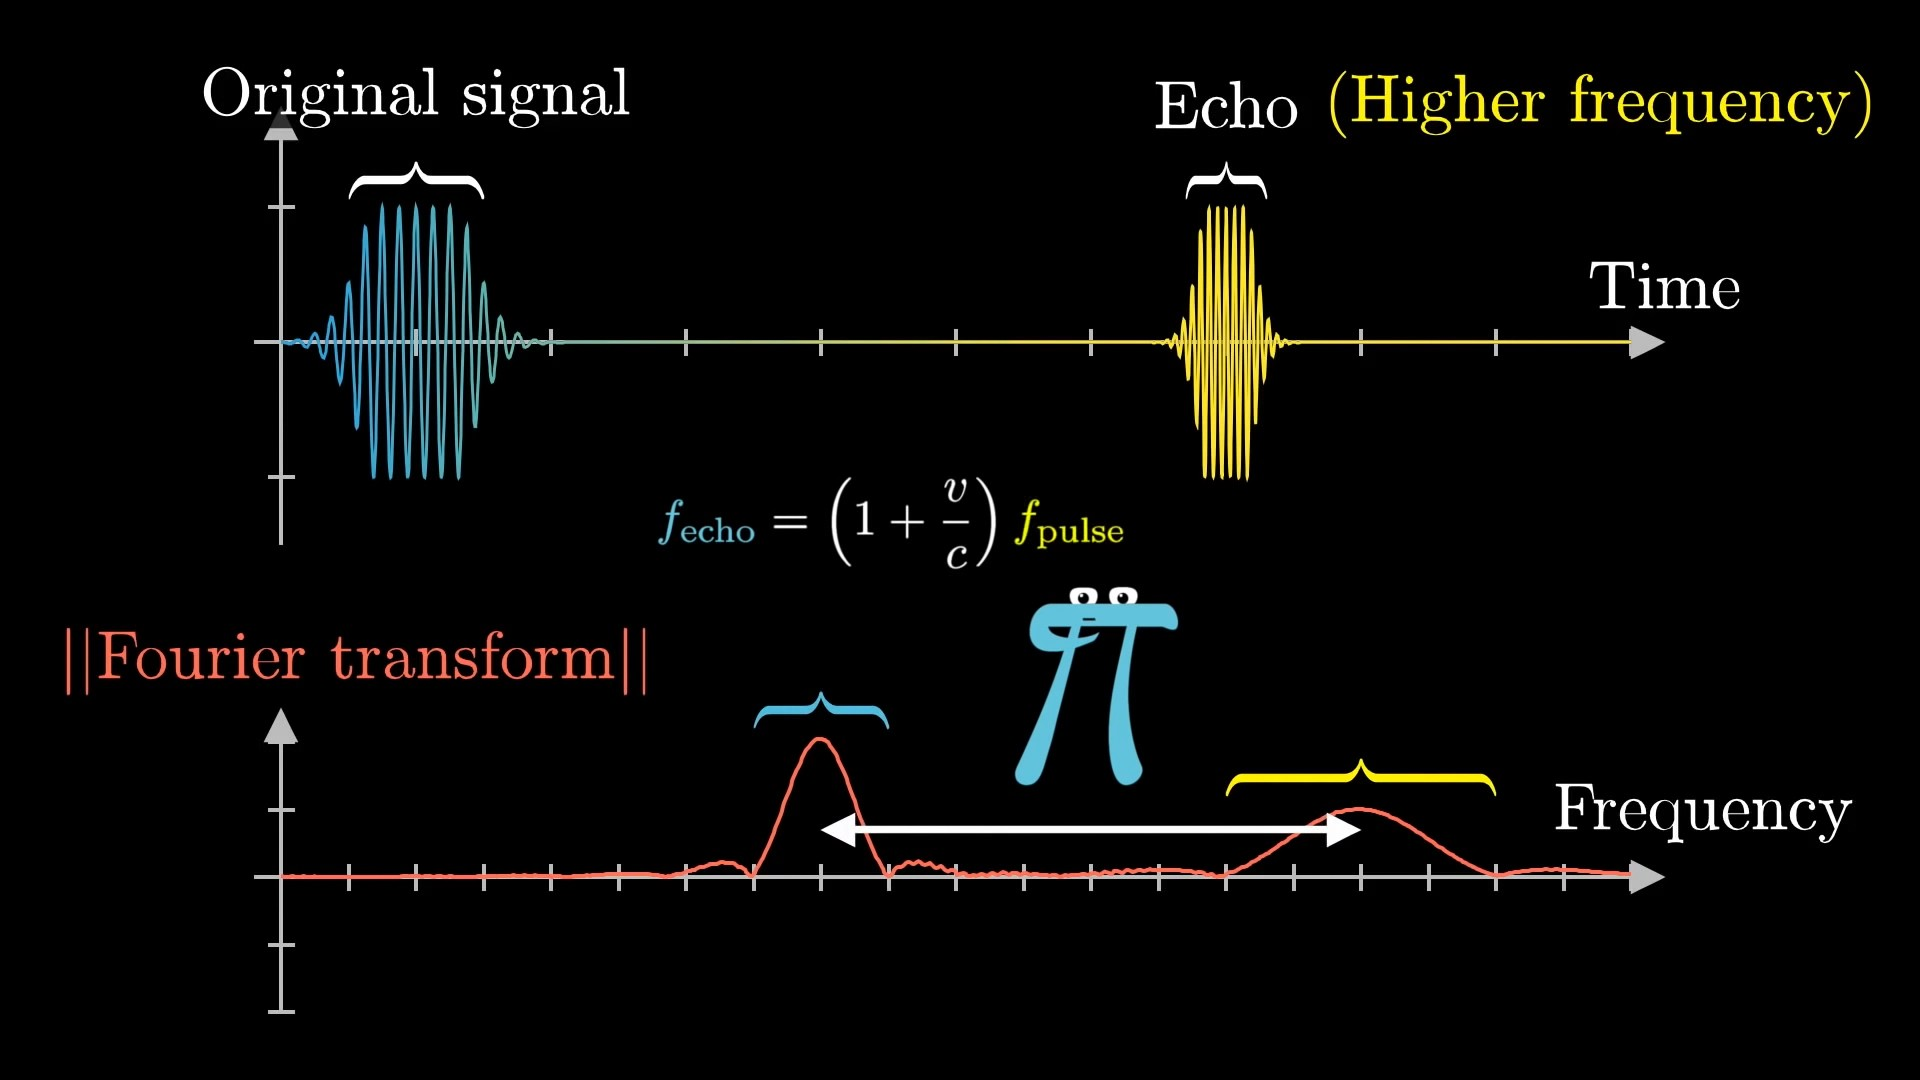
\includegraphics[scale=0.2]{env_vitesse_analyse.jpg}
	\caption{Analyse fréquentiel des signaux d'origine et de retour
	: ©3blue1brown }
\end{figure}
Ainsi par la transformée de Fourier nous obtenons suffisamment d'informations
sur le déplacement de la cible.\\
\textbf{Remarque} : Nous obtenons :
\begin{align*}
	temps &\Leftrightarrow distance \\
	fréquence &\Leftrightarrow vitesse 
\end{align*}
Ce qui est analogue au \underline{Principe d'incertitude de Heisenberg}. 


\subsection{Environnement réel}
Mais dans un environnement réel, le signal de retour est altéré. Son altération
peut être dû à des paramètres extérieur, à la qualité du radar, mais aussi le
nombre de cibles scannées. En effet, les signaux de retours peuvent s'altérer
entre eux. Donc lorsque le radar effectue un envoie long d'un signal dans un
environnement comportant une multitude de cibles, la chance d'altération est 
plus élevé.
\begin{figure}[H]
	\centering
	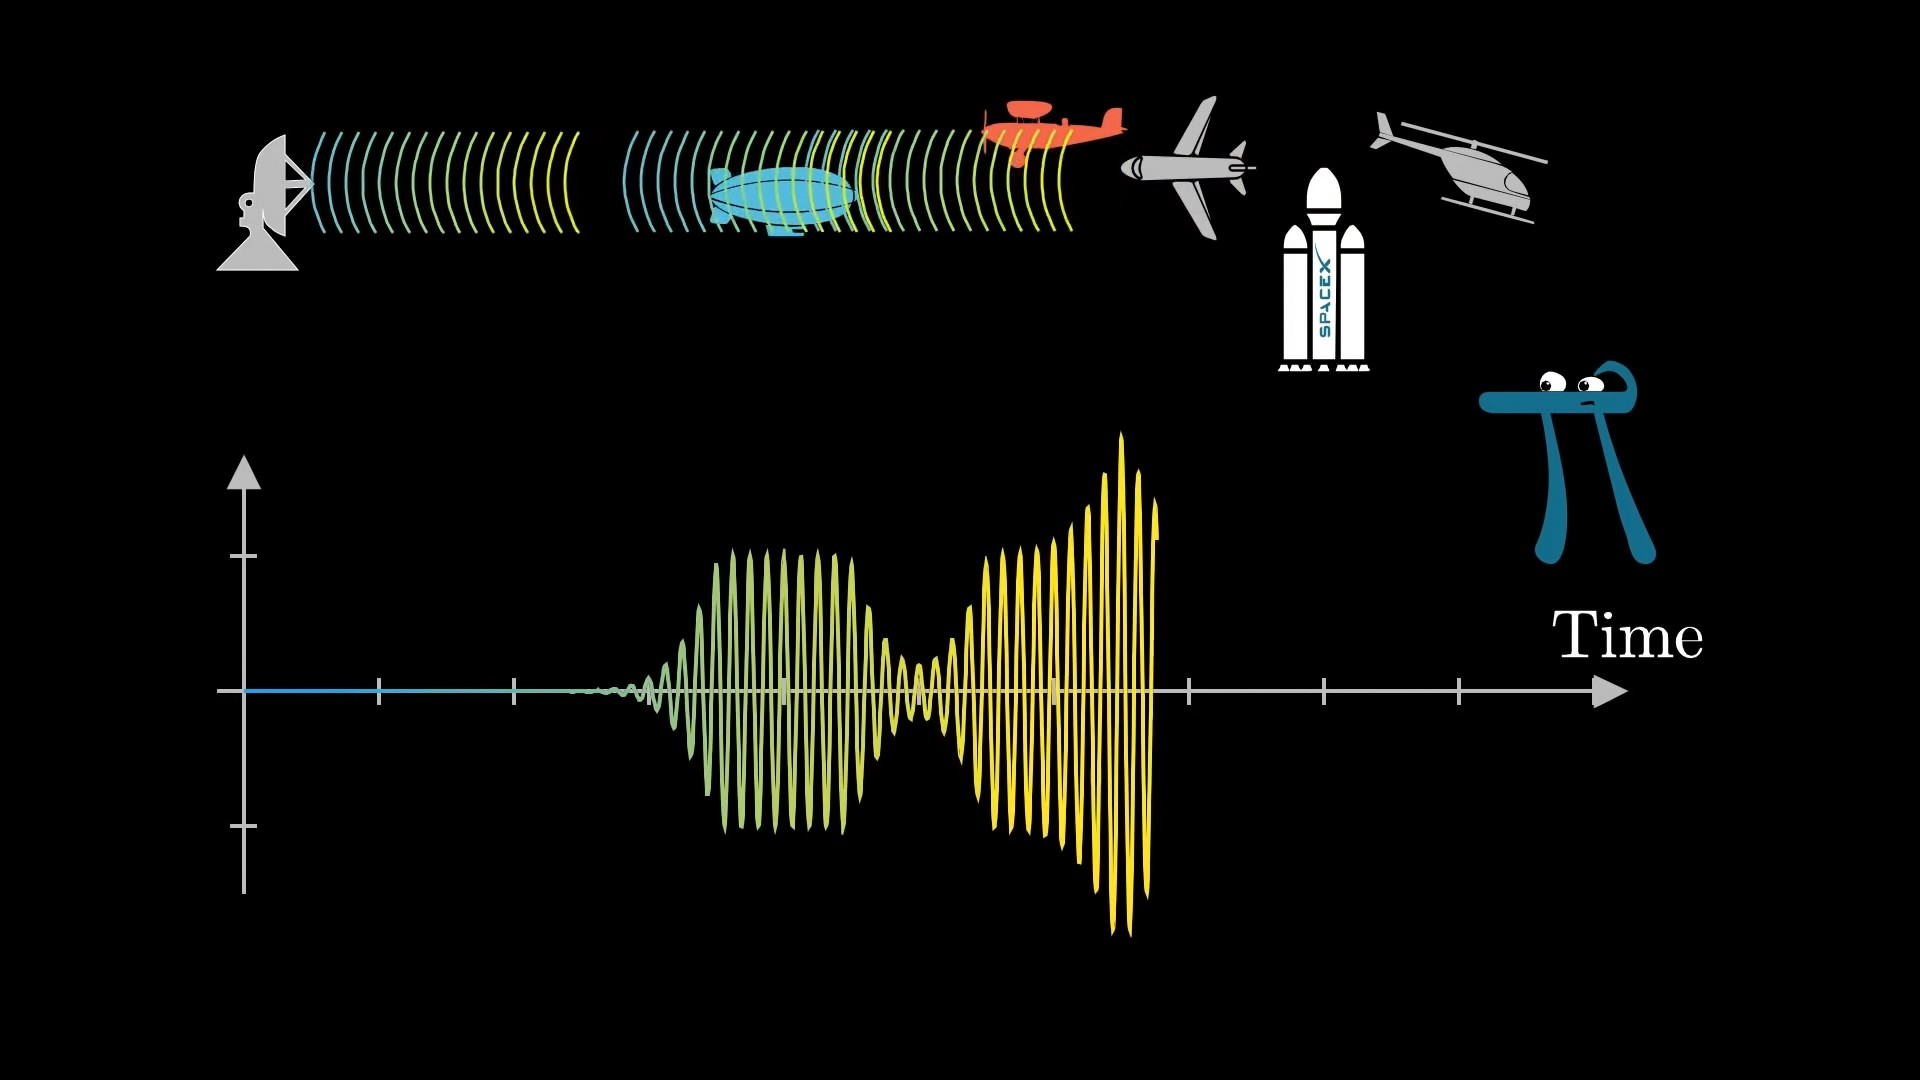
\includegraphics[scale=0.2]{env_collision.jpg}
	\caption{Collision avec multiples cibles
	: ©3blue1brown }
\end{figure}
Une des solutions est de ne pas envoyer un signal long mais de très courtes
impulsions pour ainsi en déterminer les positions de chaque cible (comme vu dans
la sous-section traitant du \textbf{Cas simple}).
\begin{figure}[H]
	\centering
	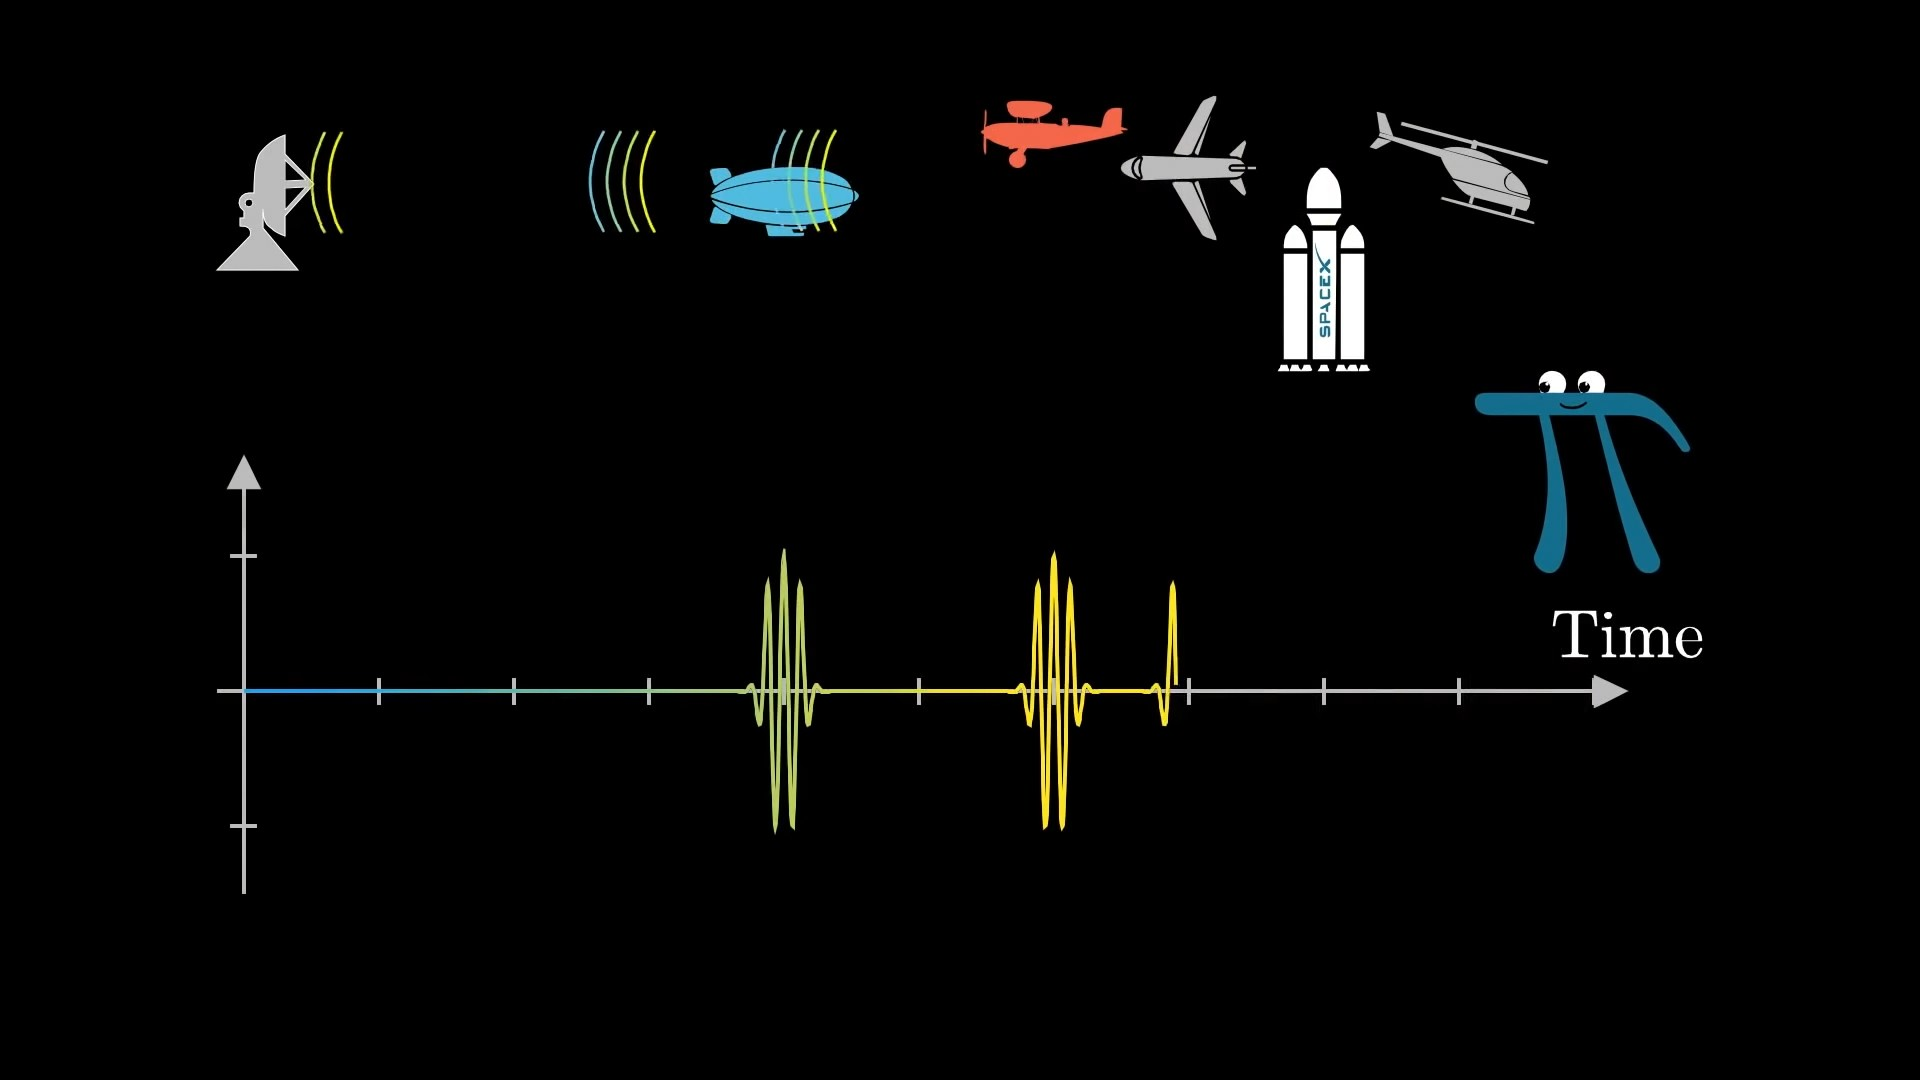
\includegraphics[scale=0.2]{env_reel_multi_simple.jpg}
	\caption{Envoie d'impulsions courtes sur multitude de cibles
	: ©3blue1brown }
\end{figure}
Lors de l'application de Fourier, étant donné, que l'impulsion est courte et par
le principe d'incertitude de Heisenberg, nous obtenons un résultat plus complexe pour
l'interprétation de la vitesse.\hfill \break
\begin{figure}[H]
	\centering
	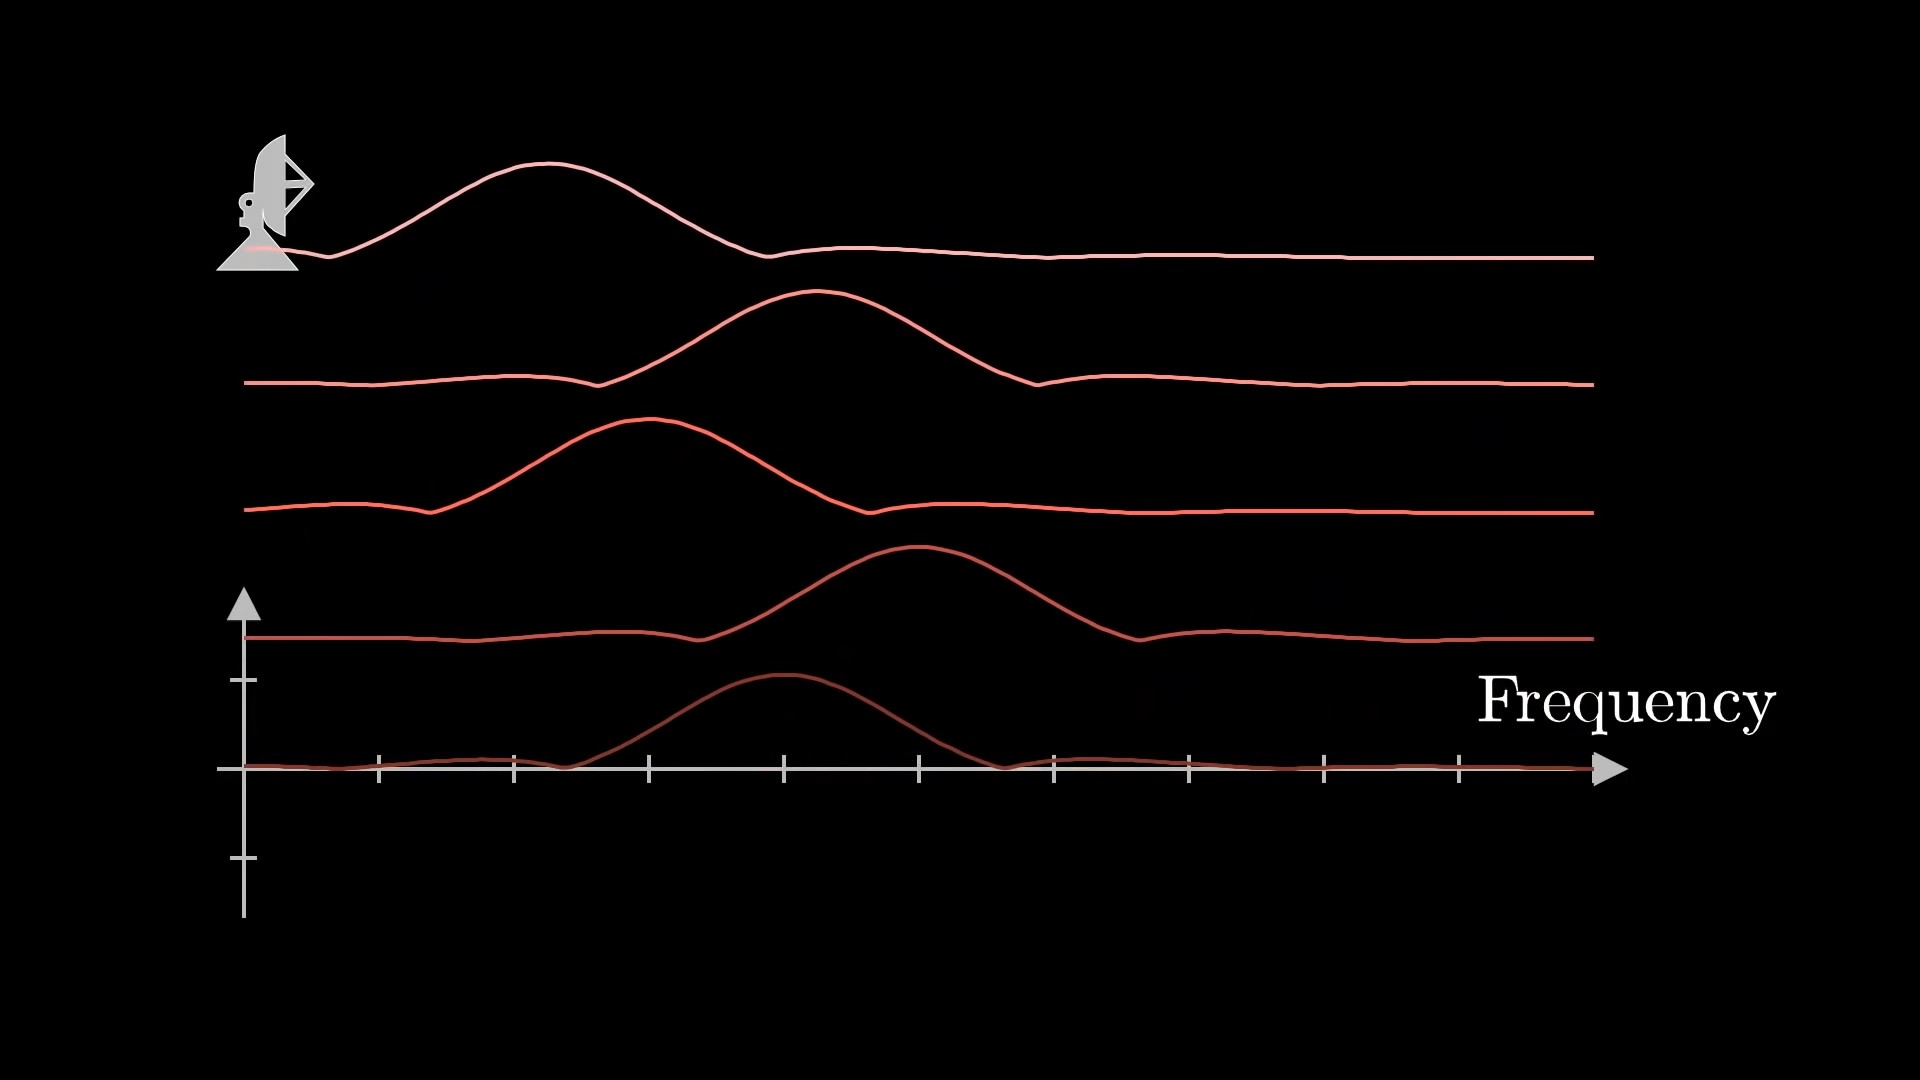
\includegraphics[scale=0.2]{conv_fourier_simple.jpg}
	\caption{Extraction des fréquences après la Transformée de Fourier des
	signaux de retours à impulsions courtes
	: ©3blue1brown }
\end{figure}
\begin{figure}[H]
	\centering
	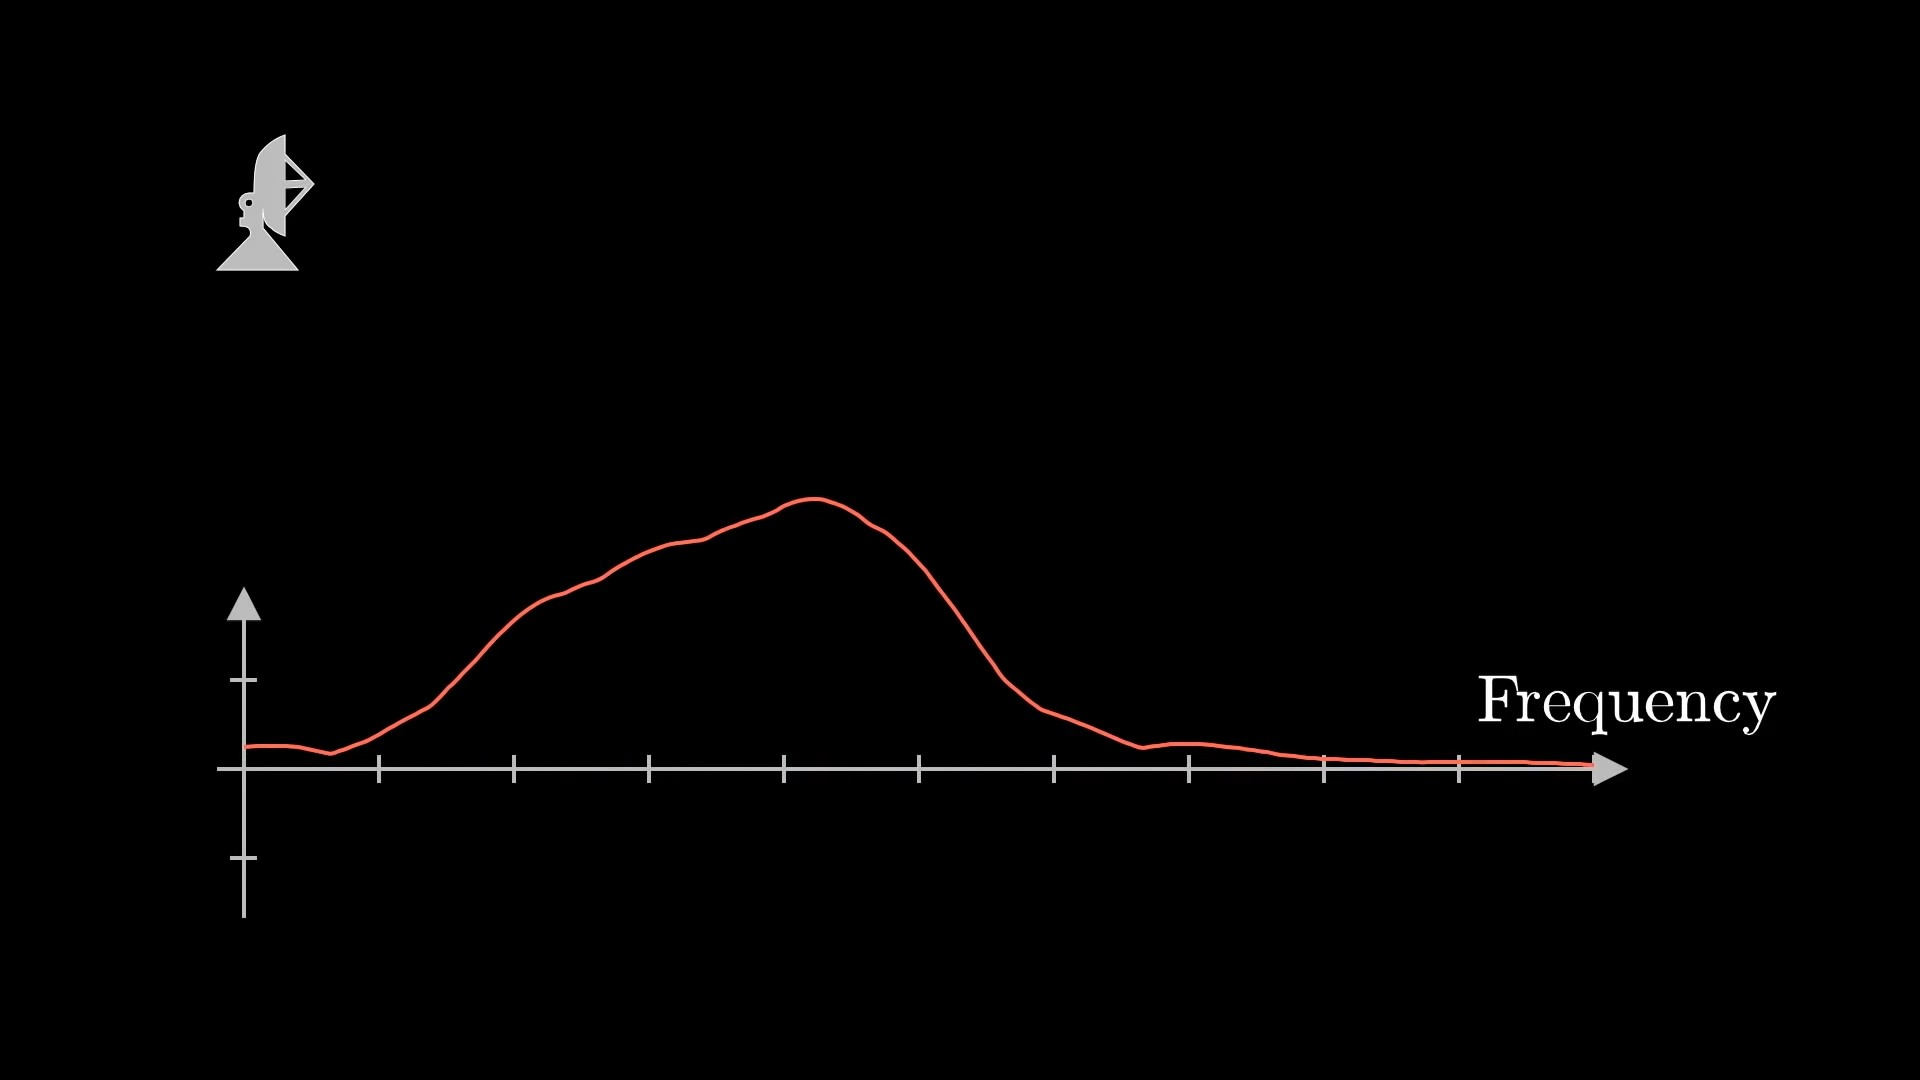
\includegraphics[scale=0.84]{somme_fourier_simple.jpg}
	\caption{Transformée de Fourier des signaux de retours à impulsion
	courtes qui démontre la complexité en l'extraction de fréquences
	indépendantes. (Il est difficile d'obtenir la décomposition comme sur la
	figure précédente.
	: ©3blue1brown }
\end{figure}




\section{Ressources}

Avant de continuer plus loins dans l'analyse de Fourier voici une série de
documents que je recommande particulièrement pour \underline{comprendre la
théorie de Fourier}, mais aussi et surtout, pour \underline{voir l'intérêt
d'étudier Fourier} :
\begin{itemize}
	\item \textbf{3blue1brown} :
		\begin{itemize}
			\item \href{https://www.youtube.com/watch?v=spUNpyF58BY}
				{3blue1brown : But what is the Fourier Transform? 
				A visual introduction.}
			\item \href{https://www.youtube.com/watch?v=r6sGWTCMz2k}{But
				what is a Fourier series? From heat flow to
				circle drawings | DE4}
			\item \href{https://www.youtube.com/watch?v=MBnnXbOM5S4}{The
				more general uncertainty principle, beyond
				quantum} (explique la relation entre la
				transformé de Fourier et le signal (au niveau
				des radars sur Doppler)). Ce qui montre que les
				chauve-souris sont capables instinctivement
				d'effectuer des Transformer de Fourier.
		\end{itemize}
	\item \textbf{Reducible} :
		\begin{itemize}
			\item \href{https://www.youtube.com/watch?v=h7apO7q16V0}{The
				Fast Fourier Transform (FFT): Most Ingenious
				Algorithm Ever?}
		\end{itemize}
	\item \textbf{SmarterEveryDay} :
		\begin{itemize}
			\item \href{https://www.youtube.com/watch?v=ds0cmAV-Yek}{
					What is a Fourier Series? (Explained by
					drawing circles) - Smarter Every Day
					205} redondant à une des vidéos de
					\textbf{3blue1brown} 
			\item \href{https://www.youtube.com/watch?v=4gibcRfp4zA}{
					Oscilloscope Music - (Drawing with
					Sound) - Smarter Every Day 224} 
					mathématiques appliqués à l'art
		\end{itemize}
	\item \textbf{Jean-Michel Bony} :
		\begin{itemize}
			\item \underline{Méthodes mathématiques pour les sciences
				physiques}. Dont la structure de ce cours est
				fortement inspirés.
		\end{itemize}
	\item \textbf{Christophe Durousseau} :
		\begin{itemize}
			\item \underline{Analyse de Fourier}
		\end{itemize}
\end{itemize}



\end{itemize}


\chapter{Fonction holomorphe d'une variable complexe}
\section{Introduction}
Dans le chapitre précédent, nous avons vu que l'on effectue un
"enroullement du signal sur le cercle unité complexe". L'exploitation de ses
données s'effectue via l'étude du point de gravité. Ce chapitre introduit les
méthodes qui en permettent son obtention.

\section{Intégral curviligne}
\emph{source :} 
\href{https://fr.wikipedia.org/wiki/Int%C3%A9grale_curviligne}{Wikipedia}

\\

En géométrie différentielle, l'\textbf{intégrale curviligne} est une intégrale où la
fonction à intégrer est évaluée sur une courbe $\Gamma$. Il y a deux types d'intégrales
curvilignes, selon que la fonction est à valeurs réelles ou à valeurs dans les
formes linéaires. Le second type (qui peut se reformuler en termes de
circulation d'un champ de vecteurs) a comme cas particulier les intégrales que
l'on considère en analyse complexe.

Dans cet article, $\Gamma$ est un arc orienté dans $\mathbb{R}^n$, rectifiable c'est-à-dire
paramétré par une fonction continue à variation bornée $t \mapsto \gamma(t)$,
avec $t \in [a,b]$. 

\subsection{Exemple}
Soit la fonction $f(z) = 1/z$, et soit $\mathrm{C}$ le cercle unité parcouru une fois dans le
sens trigonométrique, ce qui peut se paramétrer par $e^{it}$, avec $t$
parcourant $[0,2\pi]$. L'intégrale correspondante est :
\begin{equation}
	\int_{\mathrm{C}} f(z) \, dz = \int_{0}^{2\pi} \frac{1}{e^{it}} i e^{it}
	\, dt = \int_{0}^{2\pi} i \, dt = 2\pi
\end{equation}


\end{document}
